\chapter{Demystifying the Higgs Boson}

These companion notes follow Leonard Susskind's lecture on the Higgs boson and are curated by LazyingArt LLC. The lecture is deliberately narrower than the surrounding public excitement: its purpose is not to repeat the newspaper claims about the origin of the universe, but to explain, in the space of one hour, the nuts and bolts of Higgs physics. The argument proceeds in modules. It begins with quantization, fields, and vacuum structure; it then turns to spontaneous symmetry breaking in field space; only after that does it ask why the particles of the Standard Model would otherwise be massless, and how the Higgs mechanism changes that conclusion. Throughout, the pace of the lecture matters: the geometry of the bowl and the sombrero comes first, the Standard Model comes second, and the Higgs boson itself appears only after the condensate and the ``Ziggs'' mechanism are already in place.

\section{Aim and Method}

Susskind opens by rejecting the standard popular framing. The Higgs boson is indeed important, and the excitement surrounding its discovery is justified, but that is not the problem he wants to solve in this lecture. His concern is mechanical rather than ceremonial: how does Higgs physics actually work?

He also pauses at the outset to credit Fran\c{c}ois Englert and to remind the audience that the phenomenon is historically broader than the single name ``Higgs.'' In a lecture of this sort, however, he will mostly follow common usage and say ``Higgs effect.'' That remark is not incidental. It signals that the lecture will simplify where necessary, but it does not want those simplifications to erase the underlying structure.

The structure is modular. Higgs physics is, as Susskind stresses, irreducibly quantum mechanical, but he does not attempt a full course in quantum theory. Instead he isolates only the pieces he actually intends to use and builds outward from them.

\section{Quantization, Fields, and the Vacuum}

After the brief interruption near the beginning, the technical development restarts cleanly with two quantum ideas. The first is quantization. The example Susskind chooses is angular momentum:
\begin{equation}
L=n\hbar,\qquad n=0,\pm1,\pm2,\dots
\end{equation}
For the purposes of this lecture, the point is not the full theory of angular momentum, but the much simpler statement that certain physical quantities do not vary continuously. They come in discrete units.

The second quantum idea, deferred for a few minutes, is the uncertainty principle. Before returning to it, Susskind introduces the classical concept of a field.

\begin{definition}
A field is a physical quantity specified at each point of space and time. In the language of the lecture, electric, magnetic, and gravitational fields are standard examples. The vacuum is the state of lowest energy, and it need not coincide with vanishing field values.
\end{definition}

This last remark is already a quiet preparation for the Higgs story. Empty space is often imagined as a place where all fields vanish, but that is only a common expectation, not a universal requirement. One can perfectly well imagine a world in which empty space is filled with a field, just as one could imagine an electric field established by capacitor plates so far away that they are practically invisible.

The next step is to think of energy as a function of field value. If the energy is minimized at some field configuration, then that configuration is the vacuum. If the field is slightly displaced and allowed to oscillate, the oscillation is a quantum of the field. In the language Susskind repeatedly uses, the particles are quanta of field vibrations.

\section{Field-Space Potentials and Charge as Internal Motion}

For a single field component, the simplest picture is an ordinary minimum. Near that minimum, the potential may be represented schematically by
\begin{equation}
V(\phi)\propto \phi^{2}.
\end{equation}
This is not a literal board equation. It is the simplest mathematical model of the bowl-shaped geometry Susskind draws and discusses.

When more than one field component is relevant, Susskind says one may think of ``\(\phi\) and \(\phi'\).'' It is convenient to normalize that notation to a two-component field \((\phi_{1},\phi_{2})\). Then the potential is a surface over field space rather than over ordinary space:
\begin{equation}
V(\phi_{1},\phi_{2})\approx a(\phi_{1}^{2}+\phi_{2}^{2}),\qquad a>0.
\end{equation}
Again, the lecture shows the geometry rather than the formula. The essential point is rotational symmetry in field space: no matter which way the field is displaced from the origin, energy increases.

\begin{remark}
The blackboard images in this section display only the geometry of the potential and the hat analogy. The analytic formulas are standard reconstructions included to make the lecture's geometry mathematically usable.
\end{remark}

\begin{figure}
\centering
\includegraphics[width=0.78\textwidth]{lecture_144_figure_02.png}
\caption{Susskind's board sketch of the symmetric bowl together with the hat analogy used to emphasize rotational symmetry in field space.}
\end{figure}

\begin{figure}
\centering
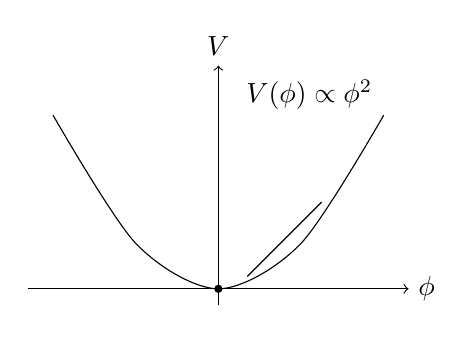
\begin{tikzpicture}[scale=1.05]
\draw[->] (-2.3,0) -- (2.3,0) node[right] {$\phi$};
\draw[->] (0,-0.2) -- (0,2.7) node[above] {$V$};
\draw plot[smooth] coordinates {(-2.0,2.1) (-1.0,0.55) (0,0) (1.0,0.55) (2.0,2.1)};
\fill (0,0) circle (0.05);
\draw (0.35,0.15) -- (1.25,1.05);
\node at (1.1,2.35) {$V(\phi)\propto \phi^2$};
\end{tikzpicture}
\caption{Editorial reconstruction of the ordinary bowl potential suggested by the board sketch. The slanted line indicates a possible displacement direction, included only as a guide to the lecture's geometry.}
\end{figure}

What matters dynamically is not only the minimum itself, but also the possibility of motion around it. If the field is displaced from the center and then set moving in a circle in field space, that motion carries an internal angular momentum. It is not angular momentum in ordinary space, but Susskind uses it as the prototype of charge. The field spins in its own internal space, and that internal rotation is quantized in the same discrete way:
\begin{equation}
L_{\mathrm{int}}=n\hbar.
\end{equation}
The lecture does not insist on a formal identification between electric charge and \(L_{\mathrm{int}}\), but it does insist on the conceptual analogy: in modern field theory, charge is naturally understood as a kind of rotation in an internal space.

\section{The Mexican Hat, Uncertainty, and the Condensate}

The decisive geometric move of the lecture is the inversion of the hat. The ordinary bowl has its minimum at the center. Now imagine turning the hat over so that the center becomes unstable and the minimum is pushed out to the brim. A standard analytic model of that geometry is
\begin{equation}
V(\phi_{1},\phi_{2})=\lambda\bigl(\phi_{1}^{2}+\phi_{2}^{2}-v^{2}\bigr)^{2},
\end{equation}
with minima satisfying
\begin{equation}
\phi_{1}^{2}+\phi_{2}^{2}=v^{2}.
\end{equation}
Thus the vacuum is no longer at zero field. The field sits somewhere on a circle of minima. One may parameterize a chosen point on that circle as
\begin{equation}
(\phi_{1},\phi_{2})=v(\cos\theta,\sin\theta).
\end{equation}

\begin{figure}
\centering
\includegraphics[width=0.72\textwidth]{lecture_144_figure_03.png}
\caption{The lecture's transition to the sombrero or Mexican-hat potential. The board shows the central peak and surrounding trough, while the hat remains part of the live analogy.}
\end{figure}

\begin{figure}
\centering
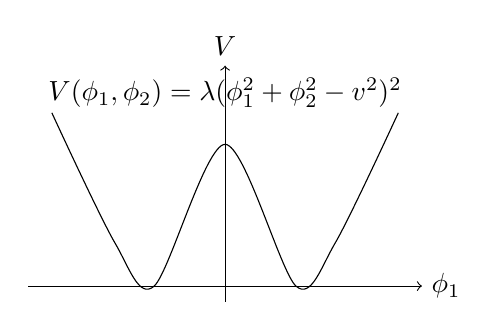
\begin{tikzpicture}[scale=1.0]
\draw[->] (-2.5,0) -- (2.5,0) node[right] {$\phi_1$};
\draw[->] (0,-0.2) -- (0,2.8) node[above] {$V$};
\draw plot[smooth] coordinates {(-2.2,2.2) (-1.4,0.55) (-0.9,0.0) (0,1.8) (0.9,0.0) (1.4,0.55) (2.2,2.2)};
\node at (0,2.45) {$V(\phi_1,\phi_2)=\lambda(\phi_1^2+\phi_2^2-v^2)^2$};
\end{tikzpicture}
\caption{Cross-sectional reconstruction of the Mexican-hat potential. The blackboard image motivates the geometry; the formula is a standard completion.}
\end{figure}

At this point the lecture draws an important classical conclusion. In the ordinary bowl, to produce rotational motion one must first displace the field from the center and then flick it around. On the brim of the Mexican hat, by contrast, motion around the trough can occur without climbing the potential. The radius stays fixed while only the angle changes. Charge-like motion has become cheap.

\begin{figure}
\centering
\includegraphics[width=0.72\textwidth]{lecture_144_figure_04.png}
\caption{The later board state in which a specific point on the trough is marked. This is the lecture's visual move from a degenerate set of minima to a chosen vacuum.}
\end{figure}

\begin{figure}
\centering
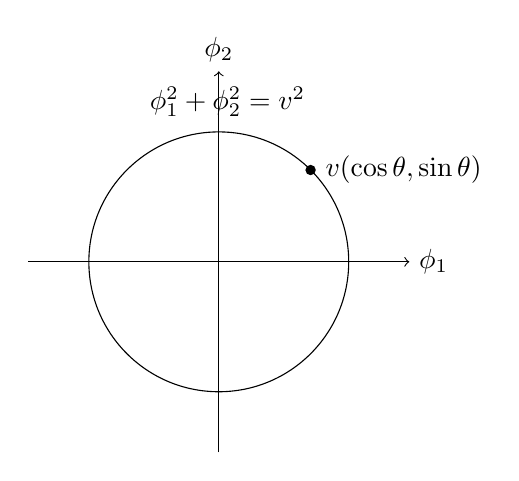
\begin{tikzpicture}[scale=1.1]
\draw[->] (-2.2,0) -- (2.2,0) node[right] {$\phi_{1}$};
\draw[->] (0,-2.2) -- (0,2.2) node[above] {$\phi_{2}$};
\draw (0,0) circle (1.5);
\fill (1.06,1.06) circle (0.06);
\node[right] at (1.12,1.06) {$v(\cos\theta,\sin\theta)$};
\node at (0.1,1.85) {$\phi_1^2+\phi_2^2=v^2$};
\end{tikzpicture}
\caption{Reconstruction of the vacuum manifold in field space. Choosing one point on the rim breaks the rotational symmetry of the potential at the level of the vacuum.}
\end{figure}

Classically, one might now say that the true vacuum is obtained by selecting one point on the rim and letting the field stand still there. Susskind's next move is to explain why quantum mechanics blocks that over-simple picture. The general uncertainty principle enters in its schematic lecture form,
\begin{equation}
\Delta x\,\Delta p \gtrsim \hbar.
\end{equation}
On the rim of the Mexican hat, the analogous statement is that a sharply localized angular position implies uncertainty in the conjugate angular motion. In the spirit of the lecture, one may formalize that idea as
\begin{equation}
\Delta\theta\,\Delta L_{\mathrm{int}} \gtrsim \hbar.
\end{equation}
Thus a vacuum sharply localized at one point on the rim cannot also have a sharply vanishing internal angular momentum or charge.

This is the point at which the classical picture becomes genuinely quantum. Empty space is no longer described as a state with a fixed charge, but as a state with indefinite charge content. Susskind's operational definition of a condensate is then simple: if one adds one quantum of the relevant charge, or removes one, nothing essential changes. The state is already so uncertain in that quantum number that such an operation merely relabels it. This is why the lecture compares the construction to a superconductor. The comparison is not ornamental; it is the main physical example of a charge condensate that already exists in familiar condensed matter physics.

\section{The Standard Model and the Mass Puzzle}

Only after the condensate story is in place does the lecture shift to what Susskind calls module number two: the Standard Model. He first reminds the audience that elementary-particle masses could in principle range all the way up to the Planck scale, but the known particles cluster extremely close to zero by that standard, around \(10^{-17}\) of the Planck mass for the heaviest known elementary particle in the lecture's 2012 setting.

The matter particles are the fermions: electrons, neutrinos, quarks, and their heavier cousins. The force-carrying particles are the bosons: the photon \(\gamma\), the gluon \(g\), and the weak bosons \(W\) and \(Z\). Susskind then presents the Standard Model dynamically, through the emission processes it allows:
\begin{align}
e &\to e+\gamma,\\
q &\to q+g,\\
f &\to f+Z.
\end{align}
The first process is ordinary electrodynamics; the second is the gluon interaction that binds quarks into hadrons; the third is the neutral weak interaction that will matter later when the \(Z\) boson enters the Higgs story.

\begin{figure}
\centering
\begin{tikzpicture}[scale=1.0]
\draw (0,0) -- (1.5,0);
\draw (1.5,0) -- (3.0,0);
\draw (1.5,0) -- (2.6,0.9);
\node at (0.45,0.25) {$e$};
\node at (2.45,-0.25) {$e$};
\node at (2.45,1.15) {$\gamma$};

\draw (4.2,0) -- (5.7,0);
\draw (5.7,0) -- (7.2,0);
\draw (5.7,0) -- (6.8,0.9);
\node at (4.65,0.25) {$q$};
\node at (6.65,-0.25) {$q$};
\node at (6.55,1.15) {$g$};

\draw (8.4,0) -- (9.9,0);
\draw (9.9,0) -- (11.4,0);
\draw (9.9,0) -- (11.0,0.9);
\node at (8.85,0.25) {$f$};
\node at (10.85,-0.25) {$f$};
\node at (10.75,1.15) {$Z$};
\end{tikzpicture}
\caption{Transcript-based reconstruction of the three emission processes Susskind uses to summarize the Standard Model.}
\end{figure}

The puzzle now becomes sharp. If this were all there was, then the particles in this stripped-down Standard Model would be massless. The photon is indeed massless, and Susskind emphasizes that the same sort of gauge-theoretic structure would also make the gluon and the \(Z\) massless. The lecture then asks why fermions would likewise fail to acquire mass, and why an additional ingredient is needed.

\section{Background Fields, Energy Shifts, and Mass Not From Higgs}

Before answering that question, Susskind inserts two carefully chosen detours. The first shows how a background field can shift energies and therefore masses. The second prevents a common overstatement by showing that much of the mass in nature has nothing to do with the Higgs mechanism.

The constructive detour is the water molecule. Treated crudely as a dipole with one positive end and one negative end, it can be placed in a uniform electric field. Outside the field, the two opposite orientations have the same mass by symmetry. Inside the field, they do not. If the dipole moment has magnitude \(d\) and the field has magnitude \(E\), then the two orientations receive opposite energy shifts:
\begin{align}
\Delta E_{\uparrow} &= -dE,\\
\Delta E_{\downarrow} &= +dE.
\end{align}
By the relation
\begin{equation}
E=mc^{2},
\end{equation}
this becomes a mass splitting:
\begin{equation}
m_{\downarrow}-m_{\uparrow}
=
\frac{\Delta E_{\downarrow}-\Delta E_{\uparrow}}{c^{2}}
=
\frac{2dE}{c^{2}}.
\end{equation}
This is the lecture's explicit worked example of a field affecting mass.

\begin{figure}
\centering
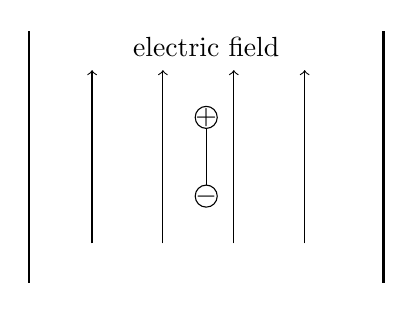
\begin{tikzpicture}[scale=1.0]
\draw[line width=1pt] (0,0) -- (0,3.2);
\draw[line width=1pt] (4.5,0) -- (4.5,3.2);
\draw[->] (0.8,0.5) -- (0.8,2.7);
\draw[->] (1.7,0.5) -- (1.7,2.7);
\draw[->] (2.6,0.5) -- (2.6,2.7);
\draw[->] (3.5,0.5) -- (3.5,2.7);
\draw (2.25,1.1) circle (0.14);
\draw (2.25,2.1) circle (0.14);
\node at (2.25,1.1) {$-$};
\node at (2.25,2.1) {$+$};
\draw (2.25,1.24) -- (2.25,1.96);
\node at (2.25,3.0) {electric field};
\end{tikzpicture}
\caption{Transcript-based reconstruction of the capacitor-field and water-dipole example. The point of the example is not drag, but an energy shift between two orientations.}
\end{figure}

Two features of the example matter. First, the field changes energy and hence mass. Second, it does so without introducing friction. This is why Susskind objects so strongly to the popular ``molasses'' analogy. The vacuum is not sticky. The molecule does not get slowed by friction; it moves through the field with no net force, while the two internal configurations simply carry different energies.

The same example can be retold in field-theoretic language. An electric field may be viewed as a condensate of photons. The water molecule then continually emits and reabsorbs photons into that condensate. Since a condensate is a state for which adding one quantum or removing one quantum does not appreciably change the background, the emitted photon may simply disappear into the condensate. The lecture represents that by a line ending in a cross.

\begin{figure}
\centering
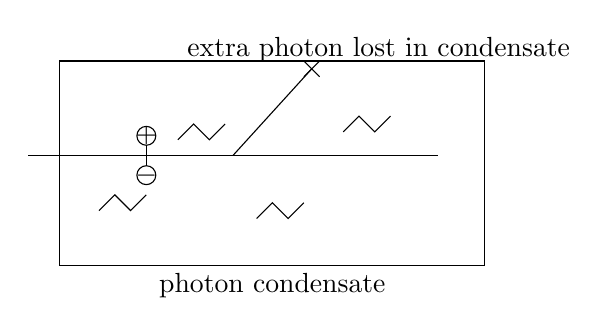
\begin{tikzpicture}[scale=1.0]
\draw (0,0.4) rectangle (5.4,3.0);
\draw (0.5,1.1) -- (0.7,1.3) -- (0.9,1.1) -- (1.1,1.3);
\draw (1.5,2.0) -- (1.7,2.2) -- (1.9,2.0) -- (2.1,2.2);
\draw (2.5,1.0) -- (2.7,1.2) -- (2.9,1.0) -- (3.1,1.2);
\draw (3.6,2.1) -- (3.8,2.3) -- (4.0,2.1) -- (4.2,2.3);
\draw (-0.4,1.8) -- (2.2,1.8);
\draw (2.2,1.8) -- (4.8,1.8);
\draw (2.2,1.8) -- (3.2,2.9);
\draw (3.10,2.80) -- (3.30,3.00);
\draw (3.10,3.00) -- (3.30,2.80);
\draw (1.1,1.55) circle (0.12);
\draw (1.1,2.05) circle (0.12);
\node at (1.1,1.55) {$-$};
\node at (1.1,2.05) {$+$};
\draw (1.1,1.67) -- (1.1,1.93);
\node at (2.7,0.15) {photon condensate};
\node at (4.05,3.15) {extra photon lost in condensate};
\end{tikzpicture}
\caption{Transcript-based reconstruction of the ``condensate of photons'' language used to reinterpret the electric field. The cross marks a quantum disappearing into the condensate.}
\end{figure}

The second detour is restrictive. Not all mass is Higgs mass. A box filled with trapped radiation behaves as a massive object simply because it stores energy:
\begin{equation}
m_{\text{box}}=\frac{E_{\text{contained}}}{c^{2}}.
\end{equation}
The proton is the lecture's key example. It is made of quarks and many gluons, and most of its mass comes from the kinetic and binding energy of those constituents rattling around inside the hadronic ``box.'' Susskind's point is strong: even if quarks and gluons were massless, the proton would lose only a tiny fraction of its mass, of order one percent in the lecture's estimate. The Higgs mechanism is therefore not a universal explanation of all mass. It is a specific explanation for the masses of the Standard Model fermions and weak bosons.

\section{Chirality, Zilch, Ziggs, and the Higgs Boson}

The lecture now narrows to the electron. Susskind does not develop the full Dirac equation, but he uses one crucial feature of Dirac theory: an electron has left-handed and right-handed chiral states, and the mass is tied to the rate at which the particle flips between them. In standard notation, that verbal statement is encoded by the Dirac mass term
\begin{equation}
m_{D}\bar\psi\psi
=
m_{D}\bigl(\bar\psi_{L}\psi_{R}+\bar\psi_{R}\psi_{L}\bigr).
\end{equation}
This formula is an editorial precision of Susskind's verbal claim that mass is the rate of left-right flipping.

\begin{figure}
\centering
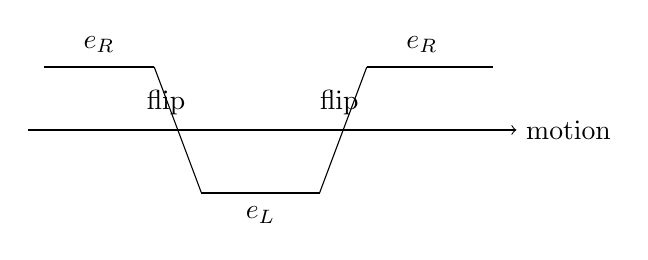
\begin{tikzpicture}[scale=1.0]
\draw[->] (0,0) -- (6.2,0) node[right] {motion};
\draw (0.2,0.8) -- (1.6,0.8);
\draw (1.6,0.8) -- (1.9,0.0);
\draw (1.9,0.0) -- (2.2,-0.8);
\draw (2.2,-0.8) -- (3.7,-0.8);
\draw (3.7,-0.8) -- (4.0,0.0);
\draw (4.0,0.0) -- (4.3,0.8);
\draw (4.3,0.8) -- (5.9,0.8);
\node at (0.9,1.08) {$e_{R}$};
\node at (2.95,-1.08) {$e_{L}$};
\node at (5.0,1.08) {$e_{R}$};
\node at (1.75,0.35) {flip};
\node at (3.95,0.35) {flip};
\end{tikzpicture}
\caption{Transcript-based reconstruction of Susskind's picture of mass as repeated left-right chirality flipping.}
\end{figure}

If the electron were strictly massless and moving at the speed of light, then in the lecture's language nothing internal could happen to it, so there would be no flipping. The electron would remain purely left-handed or purely right-handed. Why, then, is a direct left-right flip forbidden in the bare Standard Model?

The answer is the \(Z\) boson. Susskind introduces a second conserved quantity, distinct from electric charge, associated with \(Z\)-boson emission. Rather than use the standard but awkward name ``weak hypercharge,'' he invents the pedagogical label ``zilch.'' The crucial assignments in the lecture are
\begin{equation}
z(e_{L})=1,\qquad z(e_{R})=0.
\end{equation}
The left-handed and right-handed electrons have the same ordinary electric charge, but they do not have the same zilch. A direct chirality flip would therefore change a conserved quantity:
\begin{equation}
e_{L}\not\to e_{R}\qquad \text{in the bare theory.}
\end{equation}
That is why, in the stripped-down Standard Model Susskind has written on the board, the electron is massless.

The cure is the new ingredient he deliberately does \emph{not} call the Higgs boson, at least not yet. It is the ``Ziggs'' boson, a field that forms a condensate carrying indefinite zilch. Then the forbidden transition may occur in two steps:
\begin{align}
e_{L} &\to e_{R}+\mathrm{Ziggs},\\
e_{R}+\mathrm{Ziggs} &\to e_{L}.
\end{align}
Because the condensate is indifferent to the addition or removal of one Ziggs quantum, the emitted Ziggs can disappear into the condensate, or one can be pulled back out, without changing the vacuum in any observable way. Left-right mixing is restored, and with it the fermion mass.

\begin{figure}
\centering
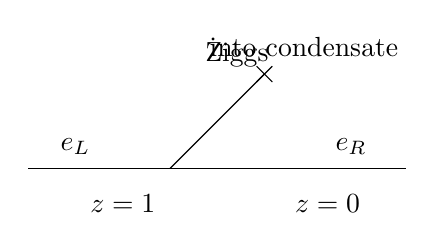
\begin{tikzpicture}[scale=1.0]
\draw (0,0) -- (1.8,0);
\draw (1.8,0) -- (4.8,0);
\draw (1.8,0) -- (3.0,1.2);
\draw (2.9,1.1) -- (3.1,1.3);
\draw (2.9,1.3) -- (3.1,1.1);
\node at (0.6,0.28) {$e_{L}$};
\node at (4.1,0.28) {$e_{R}$};
\node at (2.65,1.45) {$\mathrm{Ziggs}$};
\node at (1.2,-0.45) {$z=1$};
\node at (3.8,-0.45) {$z=0$};
\node at (3.5,1.55) {into condensate};
\end{tikzpicture}
\caption{Transcript-based reconstruction of the electron-mass mechanism in the lecture language. The electron flips chirality by emitting or absorbing a Ziggs quantum that is lost in the condensate.}
\end{figure}

Susskind immediately applies the same idea to the \(Z\) boson. Since the Ziggs carries zilch and can emit a \(Z\), the \(Z\) can exchange zilch with the condensate through the Ziggs sector and thereby behave as a massive particle. This, in the lecture's emphasis, is the Braut--Englert--Higgs phenomenon proper: the \(Z\) boson acquiring a mass from the condensate. Had the same sort of condensate existed for ordinary electric charge, the photon would have become massive as well.

\begin{figure}
\centering
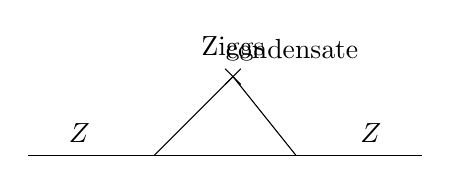
\begin{tikzpicture}[scale=1.0]
\draw (0,0) -- (5.0,0);
\draw (1.6,0) -- (2.6,1.0);
\draw (3.4,0) -- (2.6,1.0);
\draw (2.5,0.9) -- (2.7,1.1);
\draw (2.5,1.1) -- (2.7,0.9);
\node at (0.65,0.28) {$Z$};
\node at (4.35,0.28) {$Z$};
\node at (2.6,1.35) {$\mathrm{Ziggs}$};
\node at (3.35,1.35) {condensate};
\end{tikzpicture}
\caption{Transcript-based reconstruction of the analogous mechanism for the \(Z\)-boson mass. The boson mixes with condensate-supported Ziggs excitations.}
\end{figure}

Only now does Susskind say what the Higgs boson itself is. It is not the angular motion around the brim. It is the radial or density oscillation of the condensate. A standard field-theoretic reconstruction of that distinction is
\begin{equation}
\Phi(x)=(v+h(x))e^{i\theta(x)/v}.
\end{equation}
Here \(\theta(x)\) parameterizes the angular direction around the trough, while \(h(x)\) is the radial fluctuation. In the language of the lecture, \(\theta\) belongs to the Ziggs-like sector tied to the condensate, whereas \(h\) is the physical Higgs boson. Susskind gives two equivalent descriptions: \(h\) is either an oscillation in the magnitude of the field or a compression wave in the condensate density.

The short question period adds two numerical and phenomenological clarifications. First, Susskind quotes the expectation value of the Higgs field as
\begin{equation}
v\approx 240\,\mathrm{GeV}.
\end{equation}
Second, he explains that different fermions have different coupling constants to the condensate, and that these couplings control both the masses of the particles and the rates at which the Higgs decays into them. In standard notation this lecture-level statement is summarized by
\begin{equation}
g_{Hff}\propto \frac{m_{f}}{v}.
\end{equation}
Thus heavy fermions couple more strongly to the Higgs than light ones.

This brings the lecture to the question of discovery. The Higgs may decay into fermion pairs,
\begin{equation}
H\to f\bar f,
\end{equation}
and the heavier available fermions are favored. Electron-positron fusion is therefore a poor way to produce a Higgs, not because electrons cannot in principle do it, but because the coupling is weak. The top sector is much more favorable. Susskind's production story is that the Higgs is most efficiently produced by gluon fusion through a top-quark loop:
\begin{equation}
gg\to H.
\end{equation}
The same loop logic also gives the clean diphoton decay channel
\begin{equation}
H\to \gamma\gamma.
\end{equation}

\begin{figure}
\centering
\begin{tikzpicture}[scale=1.0]
\draw (0,0) -- (1.8,0);
\draw (1.8,0) -- (3.2,0.9);
\draw (1.8,0) -- (3.2,-0.9);
\node at (0.7,0.28) {$H$};
\node at (3.55,1.05) {$f$};
\node at (3.55,-1.05) {$\bar f$};
\end{tikzpicture}
\caption{Transcript-based reconstruction of Higgs decay into a fermion pair. The lecture emphasizes that heavier fermions couple more strongly.}
\end{figure}

\begin{figure}
\centering
\begin{tikzpicture}[scale=0.95]
\draw (0,1.0) -- (1.2,1.0);
\draw (0,-1.0) -- (1.2,-1.0);
\draw (1.2,1.0) -- (2.2,0);
\draw (1.2,-1.0) -- (2.2,0);
\draw (1.2,1.0) -- (1.2,-1.0);
\draw (2.2,0) -- (3.5,0);
\node at (0.45,1.25) {$g$};
\node at (0.45,-1.25) {$g$};
\node at (3.9,0.25) {$H$};
\node at (1.55,0.25) {$t$};
\node at (1.55,-0.35) {$t$};

\draw (6.2,0) -- (7.4,0);
\draw (7.4,0) -- (8.4,1.0);
\draw (7.4,0) -- (8.4,-1.0);
\draw (8.4,1.0) -- (8.4,-1.0);
\draw (8.4,1.0) -- (9.6,1.0);
\draw (8.4,-1.0) -- (9.6,-1.0);
\node at (6.65,0.25) {$H$};
\node at (9.95,1.25) {$\gamma$};
\node at (9.95,-1.25) {$\gamma$};
\node at (8.75,0.25) {$t$};
\node at (8.75,-0.35) {$t$};
\end{tikzpicture}
\caption{Transcript-based reconstructions of the two loop processes emphasized near the end of the lecture: gluon-fusion production of the Higgs through a top loop, and diphoton decay through the same loop logic.}
\end{figure}

Susskind reports the lecture-era mass value
\begin{equation}
m_{H}\approx 125\,\mathrm{GeV},
\end{equation}
and treats that as a settled fact of the 2012 discovery moment.

\begin{remark}
The lecture closes with a specifically 2012 remark about a possible excess in the diphoton decay rate, roughly a factor of \(1.5\) above the simplest expectation, at about the two-sigma level. That comment belongs to the lecture's historical horizon. Its role in the notes is to record what experimental feature Susskind told the audience to watch next, not to summarize current data.
\end{remark}

\section{Summary}

The lecture's architecture is deliberate. It does not begin with the Standard Model and only afterward mention symmetry breaking. It begins much earlier, with quantized angular momentum, fields filling space, and energy landscapes in field space. Only after the audience has seen how charge can be understood as internal rotation does Susskind turn the hat over and make the vacuum itself nontrivial.

That move produces the condensate, and the condensate produces the real payoff. In the stripped-down Standard Model, the relevant particles would be massless. The Ziggs condensate restores the forbidden left-right mixing of fermions and likewise allows the \(Z\) boson to become massive. The Higgs boson is then the remaining radial oscillation of that condensate, the density wave that was still missing experimentally in 2012.

The conceptual distinction is the one the lecture most wants to preserve: the Higgs boson is not the whole mechanism, and it is not even the first thing one should understand. First comes the field, then the Mexican-hat vacuum, then the condensate, then the mass-generating role of the Ziggs sector, and only then the Higgs boson itself as the radial mode that can be produced, decay, and be detected.